% -*- latex -*-
%%%%%%%%%%%%%%%%%%%%%%%%%%%%%%%%%%%%%%%%%%%%%%%%%%%%%%%%%%%%%%%%
%%%%%%%%%%%%%%%%%%%%%%%%%%%%%%%%%%%%%%%%%%%%%%%%%%%%%%%%%%%%%%%%
%%%%
%%%% This text file is part of the lecture slides for
%%%% `Parallel Computing'
%%%% by Victor Eijkhout, copyright 2012-2024
%%%%
%%%% ForkJoin-slides.tex : slides about OpenMP's fork-join model
%%%%
%%%%%%%%%%%%%%%%%%%%%%%%%%%%%%%%%%%%%%%%%%%%%%%%%%%%%%%%%%%%%%%%
%%%%%%%%%%%%%%%%%%%%%%%%%%%%%%%%%%%%%%%%%%%%%%%%%%%%%%%%%%%%%%%%

\begin{numberedframe}{Computer architecture terminology}
  One cluster node:

  \includegraphics[scale=.13]{stampede-node}

  A node will have 1 or 2 or (sometimes) 4 `sockets': processor
  chips.\\
  There may be a co-processor attached.
\end{numberedframe}

\begin{numberedframe}{Structure of a socket}

  \begin{multicols}{2}
    %\moveleft .5in
    \hbox{\includegraphics[scale=.25]{sandybridge-eightcore-ann}}
    \columnbreak
    \begin{itemize}
    \item Eight cores per socket, 16~per node.
    \item Access to DRAM, both this socket and other
    \item Shared L3 cache, private L2 and~L1
    \end{itemize}
  \end{multicols}
\end{numberedframe}

\begin{numberedframe}{Modern chip design}
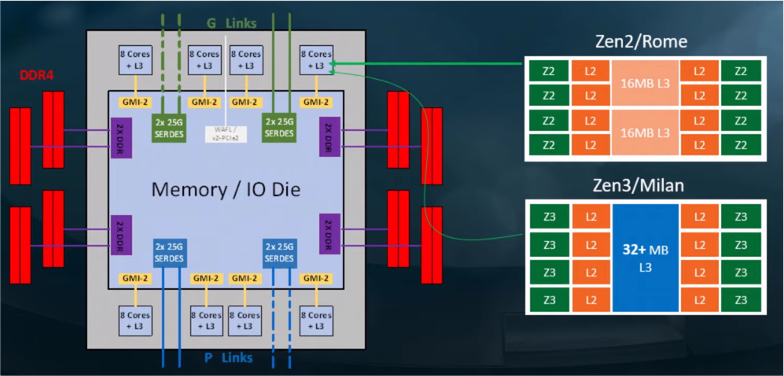
\includegraphics[scale=.5]{amd-chiplet}
\begin{itemize}
\item Shared memory
\item Shared caches
\item Local caches
\item `cc-Numa': Cache-coherent Non-Uniform Memory Access
\end{itemize}
\end{numberedframe}

\begin{numberedframe}{OpenMP history}
  \begin{itemize}
  \item First standard 1997, Fortran directives
  \item Current standard 5.2 as of 2021
  \item Intel Core processors: 2006;\\
    before that: 1980s systems from Alliant, Sequent, Denelcor;\\
    SGI Origin with up to 1024 processors\\
    supercomputers with multi-chip nodes (Intel Paragon, Cray T3D)
  \end{itemize}
\end{numberedframe}

\begin{numberedframe}{Threads}
  Process: stream of instructions\\
  Thread: process can duplicate itself, same code, access to same data

  \includegraphics[scale=.07]{fork-join}

  The OS will place threads on different cores: parallel
  performance.\\
  Note: threads are software. More threads than cores or fewer is allowed.\\
  Ignore hyperthreads
\end{numberedframe}

\begin{numberedframe}{To write an OpenMP program}
\begin{lstlisting}
#include "omp.h"
\end{lstlisting}
in C, and 
\begin{lstlisting}
use omp_lib
\end{lstlisting}
or
\begin{lstlisting}
#include "omp_lib.h"
\end{lstlisting}
for Fortran.  
\end{numberedframe}

\begin{numberedframe}{To compile an OpenMP program}
\begin{verbatim}
# gcc
gcc -o foo foo.c -fopenmp
# Intel compiler 23 and later
icc -o foo foo.c -fopenmp
# Intel compiler before 23 
icc -o foo foo.c -qopenmp
\end{verbatim}
Run as ordinary program.
\end{numberedframe}

\begin{numberedframe}{CMake}
\begin{lstlisting}
find_package(OpenMP)
# depending on language:
target_link_libraries( ${program} PUBLIC OpenMP::OpenMP_C )
target_link_libraries( ${program} PUBLIC OpenMP::OpenMP_CXX )
target_link_libraries( ${program} PUBLIC OpenMP::OpenMP_Fortran )
\end{lstlisting}
\end{numberedframe}

\begin{numberedframe}{Let's try an example}
  How many cores do we have?
\begin{lstlisting}
int omp_get_num_procs();
\end{lstlisting}
Compile and run
\end{numberedframe}

\begin{numberedframe}{Query threads}
\begin{lstlisting}
int omp_get_num_threads();
\end{lstlisting}
Compile and run. Observe?
\end{numberedframe}

\begin{numberedframe}{To run an OpenMP program}
\begin{verbatim}
export OMP_NUM_THREADS=8
./my_omp_program
\end{verbatim}
Quick experiment:
\begin{verbatim}
for t in 1 2 4 8 12 16; do
  OMP_NUM_THREADS=$t ./my_omp_program
done
\end{verbatim}
\end{numberedframe}

\begin{numberedframe}{Query threads'}
Use a parallel region:
\begin{lstlisting}[language=C]
#pragma omp parallel
{
  statements
}
\end{lstlisting}
or
\begin{lstlisting}[language=Fortran]
!$omp parallel
  statements
!$omp end parallel
\end{lstlisting}
Compile and run. Observe?
\end{numberedframe}

\begin{numberedframe}{Query threads''}
What happens if you write
\begin{lstlisting}
int t;
#pragma omp parallel
{
  t = omp_get_thread_num();
  printf("%d\n",t);
}
\end{lstlisting}
\begin{multicols}{2}
\begin{lstlisting}
{
  int t; t = // ...
  printf( ... );
}
\end{lstlisting}
\columnbreak
\begin{lstlisting}
int t;
#pragma omp parallel private(t)
\end{lstlisting}
\end{multicols}
\end{numberedframe}

\begin{exerciseframe}[parallel]
  \input{ex:omp-helloworld}
\end{exerciseframe}

\begin{exerciseframe}[parallel]
  \input{ex:omp-procthread}
\end{exerciseframe}

\begin{numberedframe}{What happens if I press that button?}
  Who of you has tried setting the number of threads (much) larger
  than the number of cores? What happened?
\end{numberedframe}

\begin{numberedframe}{Enclosed scopes}
  Data is (usually) shared in a parallel region:
  \input{sl:omp:enclosed}
  Note: this is usually the case,
  but strictly not the default.
\end{numberedframe}

\begin{numberedframe}{Thread-local variables}
  \input{sl:omp:thread-local}
\end{numberedframe}

\begin{numberedframe}{Locality of variables}
  \includegraphics[scale=.1]{fork-join-vars}
\end{numberedframe}

\begin{numberedframe}{Thread control}
  \begin{itemize}
  \item Environment variable \indexompshow{OMP_NUM_THREADS=4}
  \item Clause \indexompshow{num_threads(4)}\\
\begin{lstlisting}
#pragma omp parallel num_threads(4)
\end{lstlisting}
    usually not the best solution.
  \item Environment variable \indexompshow{OMP_THREAD_LIMIT=56}\\
    (useful for nested parallelism)
  \end{itemize}
\end{numberedframe}

\begin{numberedframe}{Limits on paralleism}
\begin{lstlisting}
#pragma omp parallel if(N>50)
\end{lstlisting}
Can you think of an application?\\
I mean, what's the harm of doing one small loop inefficiently?
\end{numberedframe}

\begin{numberedframe}{Threads and threads}
  \begin{itemize}    
  \item Threads are software, cores are hardware.
  \item The OS can move threads between cores: not a good idea for
    performance.
  \item Set: \n{export OMP_PROC_BIND=true} and you'll be good in
    most of the cases.
  \item Look up `affinity' in the OMP standard for all the details.
  \end{itemize}
\end{numberedframe}

\begin{numberedframe}{Nested parallelism}
  \input{sl:omp:nest-code}
\end{numberedframe}

\begin{numberedframe}{Nesting control}
  By default, nested levels get only one thread.\\
  Use:
\begin{lstlisting}
void omp_set_max_active_levels(int);
int omp_get_max_active_levels(void);
\end{lstlisting}
or 
\begin{verbatim}
OMP_MAX_ACTIVE_LEVELS=3
\end{verbatim}
(Deprecated: boolean switch \indexompshow{OMP_NESTED})
\end{numberedframe}

\endinput

\begin{numberedframe}{}
\begin{lstlisting}
\end{lstlisting}
\begin{itemize}
\item
\end{itemize}
\end{numberedframe}

